\documentclass{article}

\usepackage{arxiv}

\usepackage[utf8]{inputenc} % allow utf-8 input
\usepackage[T1]{fontenc}    % use 8-bit T1 fonts
\usepackage{lmodern}        % https://github.com/rstudio/rticles/issues/343
\usepackage{hyperref}       % hyperlinks
\usepackage{url}            % simple URL typesetting
\usepackage{booktabs}       % professional-quality tables
\usepackage{amsfonts}       % blackboard math symbols
\usepackage{nicefrac}       % compact symbols for 1/2, etc.
\usepackage{microtype}      % microtypography
\usepackage{graphicx}

\title{Responsible Repositories}

\author{
    Nathanael Sheehan
   \\
    College of Engineering, Mathematics and Physical Sciences \\
    Exeter University \\
  University of Exeter, St Germans Road, EX4 7HD Exeter, UK \\
  \texttt{\href{mailto:ns651@exeter.ac.uk}{\nolinkurl{ns651@exeter.ac.uk}}} \\
   \And
    Sabina Leonelli
   \\
    EGENIS, Centre For The Study Of Life Sciences \\
    Exeter University \\
  University of Exeter, St Germans Road, EX4 7HD Exeter, UK \\
  \texttt{\href{mailto:s.leonelli@exeter.ac.uk}{\nolinkurl{s.leonelli@exeter.ac.uk}}} \\
  }


% tightlist command for lists without linebreak
\providecommand{\tightlist}{%
  \setlength{\itemsep}{0pt}\setlength{\parskip}{0pt}}


% Pandoc citation processing
\newlength{\cslhangindent}
\setlength{\cslhangindent}{1.5em}
\newlength{\csllabelwidth}
\setlength{\csllabelwidth}{3em}
\newlength{\cslentryspacingunit} % times entry-spacing
\setlength{\cslentryspacingunit}{\parskip}
% for Pandoc 2.8 to 2.10.1
\newenvironment{cslreferences}%
  {}%
  {\par}
% For Pandoc 2.11+
\newenvironment{CSLReferences}[2] % #1 hanging-ident, #2 entry spacing
 {% don't indent paragraphs
  \setlength{\parindent}{0pt}
  % turn on hanging indent if param 1 is 1
  \ifodd #1
  \let\oldpar\par
  \def\par{\hangindent=\cslhangindent\oldpar}
  \fi
  % set entry spacing
  \setlength{\parskip}{#2\cslentryspacingunit}
 }%
 {}
\usepackage{calc}
\newcommand{\CSLBlock}[1]{#1\hfill\break}
\newcommand{\CSLLeftMargin}[1]{\parbox[t]{\csllabelwidth}{#1}}
\newcommand{\CSLRightInline}[1]{\parbox[t]{\linewidth - \csllabelwidth}{#1}\break}
\newcommand{\CSLIndent}[1]{\hspace{\cslhangindent}#1}

\usepackage{booktabs}
\usepackage{longtable}
\usepackage{array}
\usepackage{multirow}
\usepackage{wrapfig}
\usepackage{float}
\usepackage{colortbl}
\usepackage{pdflscape}
\usepackage{tabu}
\usepackage{threeparttable}
\usepackage{threeparttablex}
\usepackage[normalem]{ulem}
\usepackage{makecell}
\usepackage{xcolor}
\begin{document}
\maketitle


\begin{abstract}
Building on previous discussions on epistemic diversity and Open
Science, we provide a novel metric system designed to elicit information
regarding the responsibility of a given repository, as well as
documenting a clear workflow for repository maintainers to follow when
conducting this metric system. After defining the characteristics of
what constitutes as a responsible respoitory, we then use two case
studies from popular genomic survelience programs, GISAID and the
Covid-19 Data Platform, to illustrate how different interpretations of
responsible openess contribute to different implenetations of
responsibility measures. We conclude with a summary of results and a
discussion of methodological challenges and pathways for future work.
\end{abstract}

\keywords{
    Data Governance
   \and
    Data Sharing
   \and
    Open Science
   \and
    Pluralism
   \and
    SARS-CoV2
   \and
    Science Policy
  }

\newpage

\hypertarget{introduction}{%
\section{Introduction}\label{introduction}}

The pandemic disrupted normative scientific practices {[}ref{]} and
demanded rapid, scalable and open access to the latest research
findings, treatments and protocols on the coronavirus. This shift in
research practice - in conjunction with decreasing costs in data storage
- has led to an exponential increase in data repositories becoming
publicly accessible online, as well as a global recognition of Open
Science (OS) principles by the United Nations {[}REF{]}. Simultaneously,
a wider discourse emerged among policy circles and researchers with
concern to the responsibility of repositories reporting on COVID-19 and
related topics, most evidently in relation to the prompt dissemination
of genetic sequencing data from various strains of the SARS COV-2 virus
(See inter alia Meredith et al. 2020; Romano and Melo 2021, 2021; Brito
et al. 2021; Kalia, Saberwal, and Sharma 2021; Harrison et al. 2021).

On the 29th of January 2021 the governing board of the European
Bioinformatics Institute (EBI) posted a public letter in Nature calling
for a greater ``openness'' in sharing SARS-CoV-2 genome data, the letter
argued ``to unleash the fast flow of research advances'' the scientific
community must remove all formal barriers which restrict data sharing
and share all SARS-CoV-2 genome sequences to one of a triad of state
genomic surveillance programs (EBI, The GenBank of USA and the DNA Data
Bank of Japan). The letter was exclusively signed and promoted by Nobel
Laureates, Directors of Bioinformatic programs and many researchers at
the cutting edge of genome sequencing. At the same time, the Global
Initiative on Sharing Avian Influenza Data (GISAID) had just overtaken
the EBI's European COVID-19 Data Portal (C19DP) in the volume of genome
sequences being shared to open access databases (See appendix Figure 1).
GISAID was launched in 2008 to monitor global influenza outbreaks and
from the offset positioned itself as an alternative to the public domain
sharing model (creative commons), instead GISAID formulated a policy
which required users to authenticate their academic identity and agree
not to republish the sites genomes without permission from the data
producer. At the beginning of 2020, after receiving a number of
philanthropic donations from the World Health Organization, big-pharma
and nation states, GISAID launched the EpiCov database which stores,
analyses and builds evolutionary trees of SARS COV-2 genome sequences.
The platform is currently hosted by the German Institute of Agriculture
and the Max Planck institute and continues to be the leading open access
database, with over 9 million genomes sequenced.

Although the letter did not mention GISAID exclusively, this series of
events brings together a clash in ideologies on what constitutes as
responsible openness during a crisis. Leonelli (2021) introduces this
case study as a clash in ``responsible research measures,'' pointing out
how ``trustworthy and explicitly non-exploitative conditions for data
sharing helps to widen participation in data sharing.'' Under the same
logic we stipulate that trust and responsiblitlity, or a lack of it,
plays a central role in the success of OS platforms; hence researchers
and data producers alike, must ensure quality and integrity of data when
practicing OS principles in order to demonstrate the quality and
discipline which OS research demands (Azeroual and Schöpfel 2021). The
TRUST (Transparency, Responsibility, User Focus, Sustainability, and
Technology) principles put forth a set of guidelines to demonstrate the
trustworthiness of a digital repository to many of the stakeholders
involved, including researchers, community users, funders, developers
and service providers. In an OS context, a number of trustworthiness
certification mechanisms already exist;
\texttt{The\ Open\ Archival\ Information\ System} (OAIS) provides a
recommendation model to provide long-term preservation and access to
digital information (Lavoie 2004), the \texttt{FAIR} principles
emphasize a best practice of machine and human re-usability with data
objects and \texttt{datasheets\ for\ datasets} lays out a set of
questions that documents the motivation, composition, collection
process, preprocessing process, distribution and maintenance of a given
dataset (Gebru et al. 2021). Lin et al (2020) note many of these
frameworks are not suitable for a broader audience and lack a critical
understanding of the temporal aspects of a data repository, data may
enter a system under a FAIR or OAIS system, however TRUST should not be
understood as a single check box, rather it must regularly audited to
ensure the system ensures trust for the long run (Lin et al. 2020).

Building on previous discussions on epistemic diversity and Open
Science, we provide a novel metric system designed to elicit information
regarding the responsibility of a given repository, as well as
documenting a clear workflow for repository maintainers to follow when
conducting this metric system. After defining the characteristics of
what constitutes as a responsible respoitory, we then use two case
studies from popular genomic survelience programs, GISAID and the
Covid-19 Data Platform, to illustrate how different interpretations of
responsible openess contribute to different implenetations of
responsibility measures. We conclude with a summary of results and a
discussion of methodological challenges and pathways for future work.

\newpage

\hypertarget{methods}{%
\section{Methods}\label{methods}}

\hypertarget{definition}{%
\subsection{Definition}\label{definition}}

Stakeholders of a repository must take responsibility - legally and
ethically- for the data being stored and collected from their user
community. Lin et al (2020) delineates responsibility being demonstrated
as:

\begin{itemize}
\item
  "\emph{Adhering to the designated community's metadata and curation
  standards, along with providing stewardship of the data holdings
  e.g.~technical validation, documentation, quality control,
  authenticity protection, and long-term persistence.}
\item
  \emph{Providing data services e.g.~portal and machine interfaces, data
  download or server-side processing.}
\item
  \emph{Managing the intellectual property rights of data producers, the
  protection of sensitive information resources, and the security of the
  system and its content.}"
\end{itemize}

We classify our reading of responsibility into three distinct modes
which are described by sub classifications metrics. Each metric varies
on a scale from 0-1, where 0 indicates the responsibility classification
is ``not implemented,'' 0.4 indicates the responsibility classification
is ``partially implemented'' and 0.9 indicates the responsibility
classification is ``Sufficiently implemented.'' The total score for each
distinct mode is calculated as a mean weighted average from each of its
sub classifications. A summary table can be found in table 1.

\hypertarget{data-responsibility}{%
\subsection{Data Responsibility}\label{data-responsibility}}

Data Responsibility is the largest group of sub-classifications and
focuses on the quality, re-usability and interoperability of data stored
on the repository. \texttt{R1.1\ Sufficient\ Metadata} asserts
repository metadata conform to a general curation standard whereby data
can be transformed for further discoverability and provides sufficent
overviews of the data entering the platform.
\texttt{R1.2\ Technical\ Documentation} requires a closed reading of
each repository `docs,' and evaluates whether the documents provide
clear and useful instructions to successfully interact and use the
platform. \texttt{R1.3\ Format\ Control} concerns a format control test
to ensure that users uploading data have to do so in a standardized
form. \texttt{R1.4\ Content\ Control} asks if user content goes under a
form of peer review to ensure integrity of data producers.
\texttt{R1.5\ \ Database\ Authentication} checks if there are forms of
authentication in order to interact with the data repository.

\hypertarget{service-responsibility}{%
\subsection{Service Responsibility}\label{service-responsibility}}

Service Responsibility is the smallest group of sub-classifications and
focuses on the tools presented to download and upload data.
\texttt{R2.1\ Reliable\ Data\ Services} tests the performance of tools
made available to download data and further if data can be downloaded in
a range of formats and is machine readable.

\hypertarget{legal-responsibility}{%
\subsection{Legal Responsibility}\label{legal-responsibility}}

Legal Responsibility is a critical component to the R in trust as it
binds the digital and physical world.
\texttt{R3.1\ Manage\ IP\ of\ Data\ Producers} verifies the intellectual
property policy for data producers and the effects this has for both
data producers and users of the platform.
\texttt{R3.2\ Security\ of\ System} studies the vulnerabilities in
infrastructure which uphold the data, the platform and the various
microservices which contribute to the functioning of the digital system.
\texttt{R3.3\ Security\ of\ Content} describes the measures taken by
data stewards to ensure data producers content is not reshared or
published without their permission.

\begin{table}[H]

\caption{\label{tab:fig1}Modes of responsiblity and sub classifcations metrics}
\centering
\begin{tabular}[t]{l|l|l}
\hline
Data Responsibility & Service Responsibility & Legal Responsibility\\
\hline
R1.1 Curated Metadata & R2.1 Reliable Data Services & R3.1 Manage IP of Data Producers\\
\hline
R1.2 Techincal Documentation &  & R3.2 Security of System\\
\hline
R1.3 Format Control &  & R3.3 Security of Content\\
\hline
R1.4 Content Control &  & \\
\hline
R1.5  Database Authentication &  & \\
\hline
\end{tabular}
\end{table}

\newpage

\hypertarget{results}{%
\section{Results}\label{results}}

This sections outlines the justifications for each sub classification
score per case study, the full results are summarised in table 2.

\hypertarget{gisaid}{%
\subsection{GISAID}\label{gisaid}}

Overall, GISAID outperforms the Covid-19 Data Portal using our
responsibility metric. Moreover, GISAID at least partially implements
all responsibility sub classification measurements and performs best in
the Legal and Service Responsibility.

\hypertarget{data-responsibility-1}{%
\subsubsection{Data Responsibility}\label{data-responsibility-1}}

\hypertarget{r1.1-sufficient-metadata}{%
\paragraph{R1.1 Sufficient Metadata}\label{r1.1-sufficient-metadata}}

The GISAID's EpiCov database partially implements a form of standardized
metadata under the ``Submission and Variant statistics'' download
option. GISAID aid offer five meta-datasets, three of which are Excel
spreadsheets containing aggregated submissions per Country, US state or
variant; these meta-datasets are packaged in a standard wide data
format, which when transformed into a long data format contain
three/four columns: ``Country,'' ``Date,'' ``Count'' and ``Variant.'' In
addition, GISAID provide metadata concerning the variant lineage/clade
in two formats - table separate values (TSV) and JavaScript Object
Notation (JSON) - where the number of submissions is broken down by
``submissions per variant,'' ``submissions per aa substitution,''
``submissions per lineage'' and ``submissions per clade.'' While this
offers a building block in ensuring re-usability and interoperability,
all of the meta-datasets miss out on potentially useful information
which GISAID already stores for submissions, for example ``Host,''
``Location'' (at a higher spatial scale i.e city), ``originating lab''
and ``submitting lab,'' for this reason GISAID accomplishes a partially
implemented status as they are clear descripenecies in the designated
community's metadata.

\hypertarget{r1.2-techincal-documentation}{%
\paragraph{R1.2 Techincal
Documentation}\label{r1.2-techincal-documentation}}

GISAID does not provide any formal documentation on their platform, but
this is not surprising, GISAID functions solely from the graphical user
interface and does not provide any API or CLI interfaces. Instead GISAID
provides two training videos and documents on protocols.io - an open
access platform for sharing, discovering, and discussing scientific
methods - to document versions of the submission process step by step.
The quality of this documentation leads to a partial implementation
score, as the protocols and videos are only available in English and
despite the most recent protocol being the third version, it still looks
unfinished; headings are missing, there are no concluding remarks and
zero additional resources are supplied to assist in further
interoperablity.

\hypertarget{r1.3-format-control}{%
\paragraph{R1.3 Format Control}\label{r1.3-format-control}}

GISAID clearly documents a format control for data producers to follow
in order to submit sequences to the EpiCov database. This format is
accessible on both the platform and on the protocol documents. Format
control is clearly distinguished between mandatory and non mandatory
fields and provides automated checks to assert submissions do not
deviate from the existing format thus GISAID receives a sufficient
implementation score.

\hypertarget{r1.4-content-control}{%
\paragraph{R1.4 Content Control}\label{r1.4-content-control}}

Peer review is currently unknown.

\hypertarget{r1.5-database-authentication}{%
\paragraph{R1.5 Database
Authentication}\label{r1.5-database-authentication}}

One clear distinction between the two platforms is the requirement for
data producers and users to register in order to access the GISAID
database. GISAID requires users to confirm their identity and comply
with GISAID's policy to not republish data without permission from the
data producer and is the clearest distrinction between the two platforms
openess philopsohies. Authentication to the GISAID platform takes
between a few hours to several days and consists of seven ``Personal
Data'' questions (\emph{Title, Salutation, First Name, Middle Name, Last
Name, Title, Desired Login}) and eleven ``Contact information''
questions (\emph{Institution, Department, Street, Postal Code, City,
Location, State/province, Telephone, Fax, Mobile, Email}). This simple,
known and effective process determines a sufficent implementation score.

\hypertarget{service-responsibility-1}{%
\subsubsection{Service Responsibility}\label{service-responsibility-1}}

\hypertarget{r2.1-reliable-data-services}{%
\paragraph{R2.1 Reliable Data
Services}\label{r2.1-reliable-data-services}}

As previously stated, GISAID's download and upload services function
through a GUI on the platforms website. Sequences can be downloaded
using the database search page which provides an interactive environment
for querying the GISAID central database. Sequences can be filtered
using a range of drop down menus, date pickers and predefined categories
(all of which missing in the metadata, see \texttt{R1.1}) and offers
very fast sorting speeds, scoring a 92 in performance by PageSpeed
Insight tests. GISAID also provides data services to download
``Alignment and proteins,''

By not providing any other forms of tooling such as CLI or API, GISAID
partially levels the playing field in terms of accessing high volumes of
data from the GISAID database, the design of the platform does not
provide new users with the option to download the entire database. Some
researchers believe this to be an issue of differential control, however
GISAID have publicly stated this is by choice, so they have a clear
understanding of who is downloading what data and for what reasons.

. In order to download to download large col

download option which operates by calling an internal function to
trigger a data download, this implementation provides a fast download
service when the page is active and the download page scores a 92 in
performance by PageSpeed Insights.

\hypertarget{legal-responsibility-1}{%
\subsubsection{Legal Responsibility}\label{legal-responsibility-1}}

\hypertarget{r3.1-manage-ip-of-data-producers}{%
\paragraph{R3.1 Manage IP of Data
Producers}\label{r3.1-manage-ip-of-data-producers}}

The GISAID EpiCov Database utilizes a proprietary platform and software
technology which is owned by GISAID and/or third party contractors, yet
an explicit set of rules that govern the intellectual property of data
producers is logged in clause \texttt{g} of the GISAID database access
agreement. Data producers are expected to obtain the necessary
authorization or license in order to share data on GISAID and must agree
not to impose any further terms on the data which may alter or restrict
further data sharing. Moreover, data producers should not reverse
engineer or disclose any part of the database platform publiclly, as
well as not utlislising any computer viruses that may disrupt any part
of the GISAID platform. GISAID makes clear there is a
\texttt{limitation\ on\ liablity} and in no event will they be liable on
any legal grounds to lost profits, savings, data, the cost of recreating
lost data, interruption of business, or costs of procurement of
substitute goods or services. Failure to adhere to the intellectual
property agreement will lead to
\texttt{Your\ rights\ upon\ suspension\ of\ access} or
\texttt{Termination} of a users account. Although short and in sections
rather unhelpful for Data Producers, GISAID does sufficiently implement
an IP policy.

\hypertarget{r3.2-security-of-system}{%
\paragraph{R3.2 Security of System}\label{r3.2-security-of-system}}

GISAID uses a session based authentication, in contrast to token
authentication this means a session is created by the server only when a
user logged in and in GISAIDs case a session is terminated as soon as
the web page is exited or left idle for over an hour. This feature means
a base level of security is continuously running for users and data
depositors alike when using the platform. More tests could be done the
further examine the security of the system, such as Cross-Site
Scripting, SQL Injection and URL Manipulation Via HTTP GET Methods; the
authors have started to create a traceability matrix for risk and
vulnerabilities in the system, this can be accessed on request.

\hypertarget{r3.3-security-of-content}{%
\paragraph{R3.3 Security of Content}\label{r3.3-security-of-content}}

Currently unknown.

\hypertarget{covid-19-data-portal}{%
\subsection{Covid-19 Data Portal}\label{covid-19-data-portal}}

The Covid-19 Data Portal scores considerably worse than GISAID, yet this
should be understood as a difference in understanding of openess, not a
metric evaluation of right and wrong. The Covid-19 Data Portal does
provide numerous sufficient impleneteations for their genome repository
and in some cases permits for a more computationally advanced experience
when compared to GISAID.

\hypertarget{data-responsibility-2}{%
\subsubsection{Data Responsibility}\label{data-responsibility-2}}

\hypertarget{r1.1-sufficient-metadata-1}{%
\paragraph{R1.1 Sufficient Metadata}\label{r1.1-sufficient-metadata-1}}

The Covid-19 Data Portal sufficiently implements a form of stanrdisesd
metadata which contains over fifty-five data fields concerning the
sequence being submitted. Depending on the service used to download
C19DP metadata (see R2.1), metadata can be downloaded through a range of
formats, including XML, TSV, CSV and JSON and contains 55 columns (See
appendix table 3); in general C19DP metadata includes useful fields such
as ``Sex,'' ``Host,'' ``Lineage start'' and ``Lab,'' all of which
missing from GISAID, as well as some less useful such as x,y,z. One
could argue, that the C19DP metadata is much messier when compared to
GISAID, a large array of the datafields are filled as NA and column
values are not categorized to a uniform format, however this mess is
most likely the result of the various languages and definitions used
among global bioinformaticians and with a minimal data science knowledge
one can easily synthesize the data into a more useful and interporatable
format. It should also be noted that C19DP provide aggregated metadata
on a ``Statistics'' page, there is much on what can be said with regards
to the design of the charts and cartography and much the same for the
general usefulness of such simple and highly aggregated metadata.

\hypertarget{r1.3-technical-documentation}{%
\paragraph{R1.3 Technical
Documentation}\label{r1.3-technical-documentation}}

Similar to GISAID, C19DP only provides documentation in English, however
the technical docs provide a familiar format for open access software
design. Within the C19DP there exists sufficient technical documentation
for their proxy API and the bulk download tool, as well as examples on
how to formulate queries and make curl requests for each of the tools.
For data producers, C19DP links out to the ENA's SARS CoV-2 technical
documentation which provides a clear documentation for the three
submission options, GUI, CLI or submitting XML programtically via curl.
The layout of the various documentations is best suited for those
familiar with programming documentation.

. Both documentation pages can be found on the platform and each clearly

\hypertarget{r1.3-format-control-1}{%
\paragraph{R1.3 Format Control}\label{r1.3-format-control-1}}

C19DP provide format control documentation as well as automated checks
for each submission option to ensure format consistency.

\hypertarget{r1.4-content-control-1}{%
\paragraph{R1.4 Content Control}\label{r1.4-content-control-1}}

This is currently unknown.

\hypertarget{r1.5-database-authentication-1}{%
\paragraph{R1.5 Database
Authentication}\label{r1.5-database-authentication-1}}

Simply put, C19DP does not have any form of digital authentication. This
is however by design, the philosophy of the database is for rapid and
immediate access to data and would consider log-in functionality as a
barrier to data sharing. This design feature highly benefits users of
the platform, as their is no lag time between finding and accessing
potentially useful data. For data producers this lack of authentication
is blurry, data producers still have to register a sample or a study
with the ENA and EBI, which in practice is a form of authentication, by
not signing up to C19DP means data producers only have to register to
two institutions rather than three.

\hypertarget{service-responsibility-2}{%
\subsubsection{Service Responsibility}\label{service-responsibility-2}}

\hypertarget{r2.1-reliable-data-services-1}{%
\paragraph{R2.1 Reliable Data
Services}\label{r2.1-reliable-data-services-1}}

C19DP provide a REST API, GUI interface and a java bulk downloader CLI
tool, this extensive collection of tooling permits users of all
abilities to choose a method which they are most comfortable with,
however this ease of use also determines the speed and volume in which a
user can access data. For example, the GUI interface has a
\texttt{download} button where it gives the option to download a
previosuly defined query or the entire database of genome sequences - in
EMBL or FASTA format - or genome sequence metadata - in TSV or as ID's
to use with the bulk downloader, while the former works quickly the
entrire download option is rather awful, to download the full archive of
4.8 million sequences would take anything from several hours to , with
the aid of a super computer or many days while persistently having to
have a stable internet connection and not exiting the page. This
`feature' is at best tokenistic as it gives the impression that users
without a programming education may have the same data access than
someone who does, nonetheless this is a normal feature on open access
databases where the target audience is not explicitly programmers.

For those with a programming education, C19DP provide an API and a bulk
downloader CLI to speed up the process of downloading files, both tools
operate under a shared infrastructure, being the EBI search API, however
the two tools are packaged differently. C19DP API acts as a proxy for
the central European Nucleotide Archive, thereby allowing users to
efficiently query the database under a structure which fits the Covid-19
Data Portal branding. Likewise with the GUI, the API is still slow to
work with, due to the complex environment of the EBI central database
the REST API architecture has to circumnavigate many end points that
ultimately leads to slower download speeds and a less enjoyable
developer experience. The bulk downloader is certainly the most
efficient way to download large volumes of data, despite a supposedly
scary CLI, the tool allows users to download bulk batches of sequences
or metadata in parallel. The tool allows users to form queries in the
CLI, given you have the space on your computer users can retrieve tens
of gigabytes of sequence data in more formats than GISAID, this being
said, when attempting to use this tool to download the entire collection
of metadata the tool broke. These issues have been raised with the
support team at the EBI yet remained a crucial failure in repository
responsibility, with all three tools failing to download the entire
metadata it became increasingly difficult to carry out inspections of
responsibility classification. Although a solution to access a snapshot
of the latest database was offered by the EBI support team, this
solution was did not use any of the suggested C19DP data services and
instead suggested to directly use the European Nucleotide Archive.

\hypertarget{legal-responsibility-2}{%
\subsubsection{Legal Responsibility}\label{legal-responsibility-2}}

\hypertarget{r3.1-manage-ip-of-data-producers-1}{%
\paragraph{R3.1 Manage IP of Data
Producers}\label{r3.1-manage-ip-of-data-producers-1}}

It would be fair to say that C19DP is against any form of IP management
with regards to genomic surveleince of the SARS-CoV 2 Virus. C19DP
declare in the open letter only they are in the optimal position to
`achieve' the difficult task of linking Covid-19 related datasets and by
giving your faith in their resource they promise it will bring vast
benefits to societey.

\hypertarget{r3.2-security-of-system-1}{%
\paragraph{R3.2 Security of System}\label{r3.2-security-of-system-1}}

Currently unkown.

\hypertarget{r3.3-security-of-content-1}{%
\paragraph{R3.3 Security of Content}\label{r3.3-security-of-content-1}}

Due to the laissez faire IP managment, content on the C19DP is up for
grabs,

\begin{table}[H]

\caption{\label{tab:fig3}Results}
\centering
\begin{tabular}[t]{l|r|r}
\hline
Metric & GISAID: EpiCov & EBI: Covid-19 Data Platform\\
\hline
R1.1 Sufficent Metadata & 0.4 & 0.9\\
\hline
R1.2 Techincal Documentation & 0.4 & 0.9\\
\hline
R1.3 Format Control & 0.9 & 0.9\\
\hline
R1.4 Content Control & 0.9 & 0.9\\
\hline
R1.5  Database Authentication & 0.9 & 0.0\\
\hline
R2.1 Reliable Data Services & 0.9 & 0.4\\
\hline
R3.1 Manage IP of Data Producers & 0.4 & 0.0\\
\hline
R3.2 Security of System & 0.4 & 0.4\\
\hline
R3.3 Security of Content & 0.9 & 0.0\\
\hline
Total Score & 6.1 & 4.4\\
\hline
\end{tabular}
\end{table}

\hypertarget{discussion}{%
\section{Discussion}\label{discussion}}

The responsible repositories metric is intended to address the needs of
three key stakeholder groups: repository contributors, repository
consumers and repository owners. For repository contributors the metrics
identifies areas. The results from this analysis are, at best, an
attempt in deconstructing responsibility into a binary metric, the
results identify GISAID as being the more responsible database when
compared with C19DP, nonetheless responsibility as a practice is not
easily translated into numerical classifications or statistical results.
Responsibility plays out in a multitude of factors which are commonly
fogotten in purely quantitative studies, such as how practitioners of
openness interpret what counts as responsible openness or how different
community users acknowledge and interact with each platform. Without
coupling a quantitative measurements with qualitative experience.
Further work refining the binary metric system may serve as a robust
piece of empirical contribution in understanding the general question of
responsibility in respotistiores, however only when coupled with
qualitative differences.

The debate over GISAID and its governance structure exemplifies how
efforts to abide by the principle of openness, particularly when it
comes to Open Data, can clash with responsible research measures geared
towards protecting researchers whose work is unrecognised and/or
discriminated against. In this as in many other cases, providing
trustworthy and explicitly non-exploitative conditions for data sharing
helps to widen participation in data sharing, which in turn expands the
evidence base for subsequent discoveries. It also helps prevent the
circulation of low-quality data (Leonelli 2018a), the expansion of
digital divides (Bezuidenhout et al 2017) and socially harmful research
(Elliott and Resnik 2019). In choosing to sidestep these issues,
researchers calling for ``fully open'' data are discounting the
significance of socio-cultural factors (such as the geo-political
location and characteristics of researchers), institutional issues (such
as power dynamics among research sites, expectations around intellectual
property) and infrastructural resources (such as the availability of
funding and dependable connectivity) to data re-use. Paradoxically, this
may result in excluding some researchers from data sharing
initiatives,which reduces the diversity and range of data available
online, thereby constraining the evidence base for evaluating existing
knowledge claims and developing new ones.

\begin{enumerate}
\def\labelenumi{(\arabic{enumi})}
\setcounter{enumi}{4}
\tightlist
\item
  discuss how this works out in case og GISAID vs COVID-19 portal: here
  we have a clash of ideologies and experiences of what constitutes
  ``good'' openness
\end{enumerate}

\hypertarget{conclusion}{%
\section{Conclusion}\label{conclusion}}

\begin{enumerate}
\def\labelenumi{(\arabic{enumi})}
\setcounter{enumi}{5}
\tightlist
\item
  conclusion: there is much that CAN be done to metricise and evaluate
  TRUST principles as a key complement to FAIR, however even such
  evaluation needs to highlight the unavoidable
  qualitative/interpretative differences in the implementation of
  openness
\end{enumerate}

\hypertarget{appendix}{%
\section{Appendix}\label{appendix}}

\begin{figure}
\centering
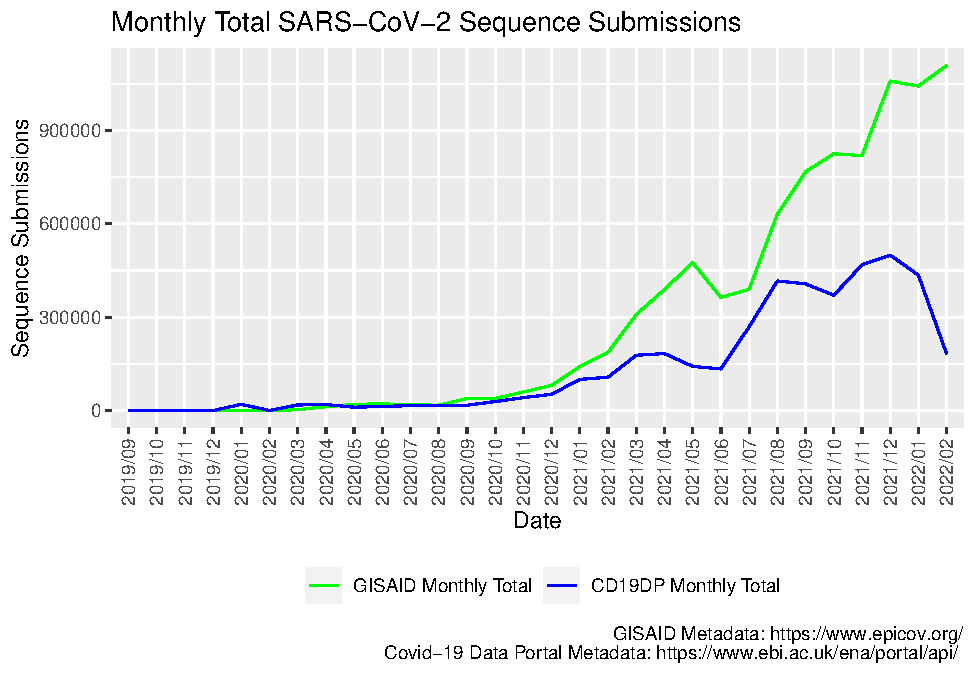
\includegraphics{Report_files/figure-latex/fig2-1.pdf}
\caption{Monthly totals of global SARS-CoV-2 cases sequenced and shared
on the GISAID and Covid-19 Data Platform database until Febuary 22 2022}
\end{figure}

\hypertarget{references}{%
\section*{References}\label{references}}
\addcontentsline{toc}{section}{References}

\hypertarget{refs}{}
\begin{CSLReferences}{1}{0}
\leavevmode\hypertarget{ref-AZEROUAL2021169}{}%
Azeroual, Otmane, and Joachim Schöpfel. 2021. {``18 - Trustworthy or
Not? Research Data on COVID-19 in Data Repositories.''} In
\emph{Libraries, Digital Information, and COVID}, edited by David Baker
and Lucy Ellis, 169--82. Chandos Digital Information Review. Chandos
Publishing.
https://doi.org/\url{https://doi.org/10.1016/B978-0-323-88493-8.00027-6}.

\leavevmode\hypertarget{ref-Brito2021}{}%
Brito, Anderson F, Elizaveta Semenova, Gytis Dudas, Gabriel W Hassler,
Chaney C Kalinich, Moritz U G Kraemer, Sarah C Hill, et al. 2021.
{``Global Disparities in SARS-CoV-2 Genomic Surveillance.''}
\emph{medRxiv : The Preprint Server for Health Sciences}, August.
\url{https://doi.org/10.1101/2021.08.21.21262393}.

\leavevmode\hypertarget{ref-Gebru2021}{}%
Gebru, Timnit, Jamie Morgenstern, Briana Vecchione, Jennifer Wortman
Vaughan, Hanna Wallach, Hal Daumé III, and Kate Crawford. 2021.
{``Datasheets for Datasets.''} \emph{Communications of the ACM} 64
(December): 86--92. \url{https://doi.org/10.1145/3458723}.

\leavevmode\hypertarget{ref-Harrison2021}{}%
Harrison, Peter W, Rodrigo Lopez, Nadim Rahman, Stefan Gutnick Allen,
Raheela Aslam, Nicola Buso, Carla Cummins, et al. 2021. {``The COVID-19
Data Portal: Accelerating SARS-CoV-2 and COVID-19 Research Through Rapid
Open Access Data Sharing.''} \emph{Nucleic Acids Research} 49 (July):
W619--23. \url{https://doi.org/10.1093/nar/gkab417}.

\leavevmode\hypertarget{ref-Kalia2021}{}%
Kalia, Kishan, Gayatri Saberwal, and Gaurav Sharma. 2021. {``The Lag in
SARS-CoV-2 Genome Submissions to GISAID.''} \emph{Nature Biotechnology}
39 (September): 1058--60.
\url{https://doi.org/10.1038/s41587-021-01040-0}.

\leavevmode\hypertarget{ref-lavoie2004open}{}%
Lavoie, Brian F. 2004. {``The Open Archival Information System Reference
Model: Introductory Guide.''}

\leavevmode\hypertarget{ref-pittphilsci19817}{}%
Leonelli, Sabina. 2021. {``Open Science and Epistemic Diversity: Friends
or Foes?''} In. \url{http://philsci-archive.pitt.edu/19817/}.

\leavevmode\hypertarget{ref-Lin2020}{}%
Lin, Dawei, Jonathan Crabtree, Ingrid Dillo, Robert R. Downs, Rorie
Edmunds, David Giaretta, Marisa De Giusti, et al. 2020. {``The TRUST
Principles for Digital Repositories.''} \emph{Scientific Data} 7
(December): 144. \url{https://doi.org/10.1038/s41597-020-0486-7}.

\leavevmode\hypertarget{ref-Meredith2020}{}%
Meredith, Luke W, William L Hamilton, Ben Warne, Charlotte J Houldcroft,
Myra Hosmillo, Aminu S Jahun, Martin D Curran, et al. 2020. {``Rapid
Implementation of SARS-CoV-2 Sequencing to Investigate Cases of
Health-Care Associated COVID-19: A Prospective Genomic Surveillance
Study.''} \emph{The Lancet Infectious Diseases} 20 (November): 1263--71.
\url{https://doi.org/10.1016/S1473-3099(20)30562-4}.

\leavevmode\hypertarget{ref-Romano2021}{}%
Romano, Camila M, and Fernando L Melo. 2021. {``Genomic Surveillance of
SARS-CoV-2: A Race Against Time.''} \emph{The Lancet Regional Health -
Americas} 1 (September): 100029.
\url{https://doi.org/10.1016/j.lana.2021.100029}.

\end{CSLReferences}

\bibliographystyle{unsrt}
\bibliography{references.bib}


\end{document}
